\documentclass[tikz,border=4pt]{standalone}
\usepackage{pgfplots}
\pgfplotsset{compat=1.17}
\begin{document}
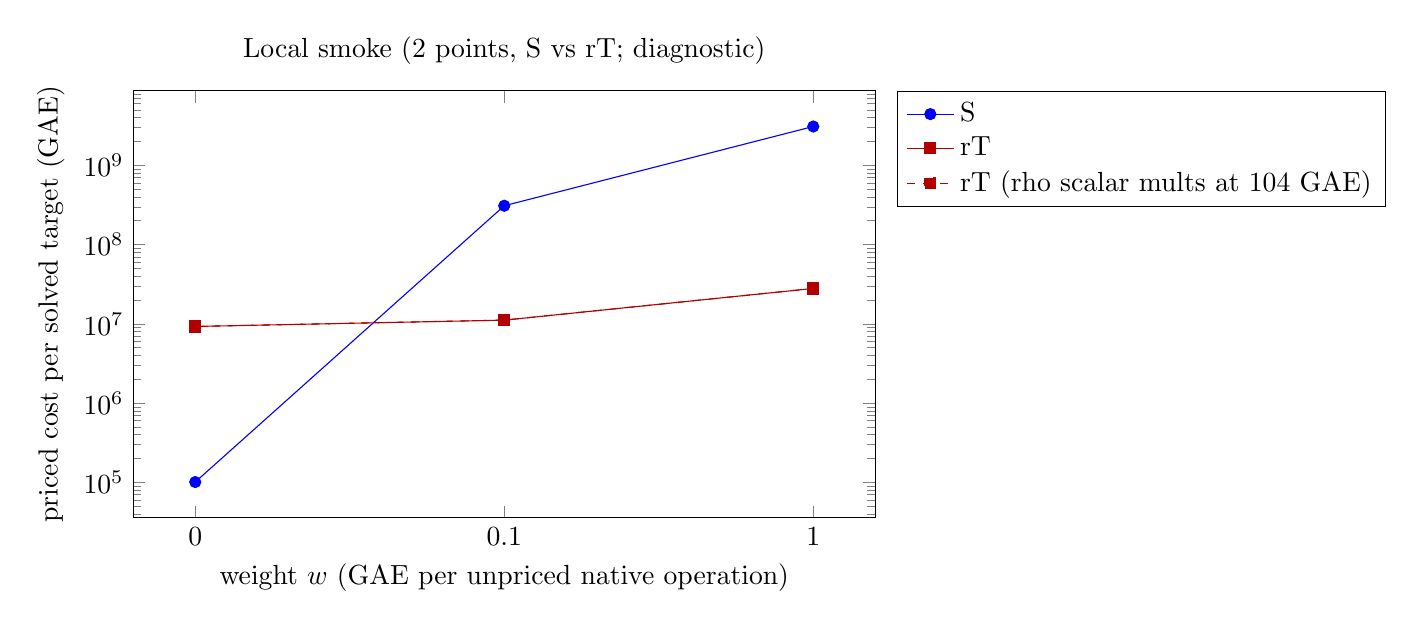
\begin{tikzpicture}
\begin{axis}[width=11cm, height=7cm, ymode=log, xlabel={weight $w$ (GAE per unpriced native operation)},
  ylabel={priced cost per solved target (GAE)}, xtick={0,1,2}, legend pos=outer north east,
  xticklabels={0,0.1,1}, title={Local smoke (2 points, S vs rT; diagnostic)}, legend cell align=left]
\addplot[blue, mark=*] coordinates {(0,101084) (1,3.0936e+08) (2,3.09269e+09)};
\addlegendentry{S}
\addplot[red!70!black, mark=square*] coordinates {(0,9.27971e+06) (1,1.115e+07) (2,2.79824e+07)};
\addlegendentry{rT}
\addplot[red!70!black, mark=square*, dashed] coordinates {(0,9.28335e+06) (1,1.11536e+07) (2,2.7986e+07)};
\addlegendentry{rT (rho scalar mults at 104 GAE)}
\end{axis}
\end{tikzpicture}
\end{document}
